\documentclass[12pt,a4paper]{article}

% Margins.
\setlength{\oddsidemargin}{0in}
\setlength{\evensidemargin}{0in}
\setlength{\headheight}{12pt}
\setlength{\headsep}{42pt}
\setlength{\topmargin}{-54pt}
\setlength{\textwidth}{6.5in}
\setlength{\textheight}{10in}

\usepackage{amsmath}
\usepackage{float}
\usepackage{graphicx}
\usepackage[hyphens]{url}
\usepackage{hyperref}	% Clickable links to figures, references and urls.
\usepackage{datetime}
\usepackage{longtable}
\usepackage{subfigure}

% Links direct to top of figures.
\usepackage[all]{hypcap}

% Drawing.
\usepackage{pgf}
\usepackage{tikz}

% Listings for formatting code.
\usepackage{listings}
\usepackage{textcomp}
% General options.+++
\lstset{breaklines=true, basicstyle=\small\ttfamily, tabsize=4, numbers=left, stepnumber=1, frame=single, showstringspaces=false, upquote=true}
% C++ specific high-lighting. Comments are 50/50 shades of green/black and strings coloured with 60/40 red/black mixture.
\lstset{language=[ISO]C++, commentstyle=\color{green!50!black}, keywordstyle=\color{blue}, stringstyle=\color{red!60!black}}

%opening
\title{\vspace{-2cm}Physics for Engineers\\Class 18\\Continuous Charge Distributions}
\author{Attique Dawood}
\date{March 06, 2014\\[0.2cm] Last Modified: \today, \currenttime}
\begin{document}
\maketitle
\section{Announcements}
\begin{itemize}
\item None.
\end{itemize}
\section{Continuous Charge Distributions}
In real life charges mostly appear bunched in different formations resembling the shape of the object on which they reside. It is more practical to think of continuous charge distributions rather than individual point charges.

Here we define three charge distributions, the line charge density, surface charge density and volume charge density. For uniform charge densities over and entire length, area or volume,
\begin{equation}
\rho_L=\dfrac{Q}{L},
\end{equation}
\begin{equation}
\rho_S=\dfrac{Q}{A},
\end{equation}
and
\begin{equation}
\rho_V=\dfrac{Q}{V}.
\end{equation}
Here Q is the total charge spread over length L, surface S or volume V. If the charge distribution is not uniform we can define differential charge as
\begin{equation}
dq=\rho_Ldl,
\end{equation}
\begin{equation}
dq=\rho_SdS,
\end{equation}
and
\begin{equation}
dq=\rho_Vdv.
\end{equation}
Integration of differential charge expression gives the total charge.
Note: Serway and Jewet \cite{Serway} refer to these charge densities as $\lambda$, $\sigma$ and $\rho$.
\section{Exercises}
\noindent\textbf{Question 1 \cite[Example 23.7, page 721]{Serway}:} A rod of length $L$ has a uniform positive charge per unit length $\lambda$ or $\rho_l$ and a total charge $Q$. Calculate the electric field at a point $P$ that is located along the long axis of the rod and a distance $a$ from one end (figure \ref{electric-field-charged-rod}).
\begin{figure}[H]
\centering
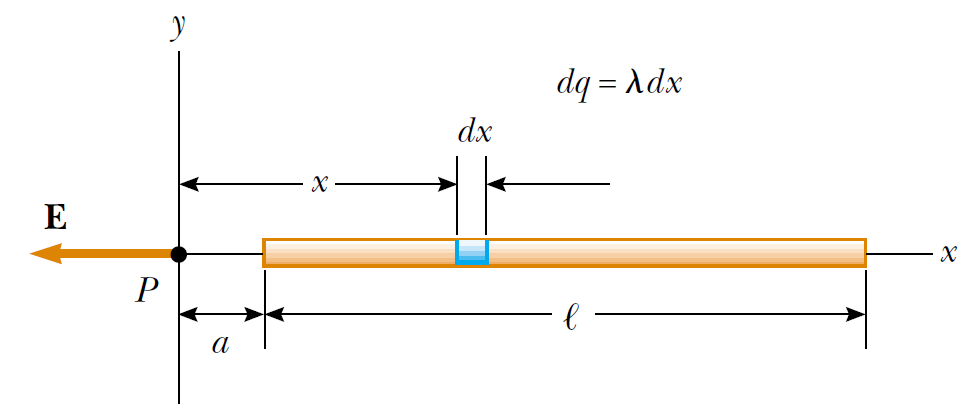
\includegraphics[scale=0.45]{Figure23-17.png}
\caption{Electric field of a charged rod.}
\label{electric-field-charged-rod}
\end{figure}
\noindent\textbf{Question 2 \cite[Problem 4.5, page 155]{Sadiku}:} Determine the total charge for the following non--uniform charge distributions.
\begin{itemize}
\item[a.] On line $0 < x < 5$ m if $\rho_L$ or $\lambda$ = $2x^2$ mC/m.
\item[b.] On the surface of cylinder defined by $\rho$ = 3, $0 < z < 4$ m if $\rho_S$ = $\rho z^2$ nC/m$^2$.
\item[c.] Within the sphere $r = 4$ m if $\rho_V$ = $\dfrac{10}{r\sin\theta}$ C/m$^3$.
\end{itemize}
%\nocite{*}
\bibliographystyle{plain}
\bibliography{PhysicsRef}
\end{document}
